\documentclass[conference]{IEEEtran}
% 9th ABC Challenge — head-pose prediction. Compile with pdflatex (Overleaf: IEEE Conference template).
\usepackage{amsmath,amssymb}
\usepackage{graphicx}
\usepackage{booktabs}
\usepackage{multirow}
\usepackage{xcolor}
\usepackage{tikz}
\usetikzlibrary{positioning,arrows.meta,fit}
\usepackage[hidelinks]{hyperref}
\newcommand{\todo}[1]{\textcolor{red}{[TODO: #1]}}
\newcommand{\ours}{HeadFormer}   % model name — rename freely

\begin{document}

\title{\ours: A 122k-Parameter Motion-Token Transformer\\for Zero-Shot Head-Pose Prediction on XR Edge Devices}

\author{
\IEEEauthorblockN{\todo{Author 1}, \todo{Author 2}, \todo{Author 3} \todo{(all team members)}}
\IEEEauthorblockA{\todo{Affiliation}\\
\todo{Team name: TEAMNAME} \quad \todo{e-mail}}
}

\maketitle

\begin{abstract}
Extended-reality (XR) headsets must render for where the user's head \emph{will} point, not where it pointed when the frame
was started. For the 9th ABC Challenge we predict the next 20 head orientations (200\,ms at 100\,Hz) from a window of past
quaternions, for unseen users and under tight edge-deployment budgets. We present \ours, a compact transformer that
(i) converts quaternions into heading-invariant motion features (head-frame angular velocity, tilt, speed and angular
acceleration), (ii) groups them into 50\,ms patch tokens with a recency embedding and a readout token, and (iii) predicts a
residual on top of a learned constant-velocity prior, trained directly on the challenge's geodesic metric. Trained on
10{,}677 BOXRR-23 users and evaluated on 46{,}474 windows from 1{,}330 held-out users, \ours\ reaches a mean error of
4.52$^\circ$ at the 20th sample---39.6\% below the mandated constant-velocity baseline and 19.1\% below a tuned
damped-velocity model---with 121{,}892 parameters, 2.2\,M MACs per prediction and 0.25\,ms CPU latency. A controlled
benchmark of 13 predictors (physics baselines, GRU/LSTM/TCN/SSM, KalmanNet, QuaterNet, MOUNT, controlled residual learning
and a 1.3\,M-parameter GRT-style transformer) shows that all learned models except KalmanNet lie within 0.5$^\circ$ of each other, that
the remaining error is dominated by motion onsets that the past head trajectory cannot reveal, and that at this point
efficiency rather than capacity separates good from best.
\end{abstract}

\begin{IEEEkeywords}
head-pose prediction, extended reality, quaternions, transformers, edge AI, BOXRR-23
\end{IEEEkeywords}

% =====================================================================================================
\section{Introduction}
Motion-to-photon latency remains a central problem in XR: every millisecond between sensing the head pose and displaying the
corresponding image shows up as swimming or lag. Rendering for a \emph{predicted} pose hides part of this latency, and pose
prediction has been part of head-tracking pipelines from the start~\cite{azuma1995,lavalle2014}. Classical predictors
extrapolate the current motion (constant velocity, Kalman filters); learned predictors promise to capture the structure of
human head movement, but are usually trained on small, task-specific datasets.

The 9th ABC Challenge asks for a single model that, given up to 400 past head-orientation quaternions sampled at 100\,Hz,
predicts the next 20 orientations\footnote{The challenge page describes the 20 outputs as ``100 milliseconds''; at 100\,Hz,
20 samples span 200\,ms, which is the horizon we evaluate. \todo{confirm with organisers if needed}}, generalises zero-shot
to unseen users, and runs on an XR edge platform. Submissions are ranked on accuracy (40\%), latency (30\%), parameter
count (10\%) and innovation (20\%); accuracy is the mean geodesic error of the 20th predicted sample,
\begin{equation}
\theta = 2\arccos\bigl|\langle \hat{q}_{t+20},\, q_{t+20}\rangle\bigr| .
\label{eq:metric}
\end{equation}
Because three of the four criteria reward small and fast models, we treat efficiency as a first-class design goal rather
than an afterthought.

\textbf{Contributions.}
\begin{itemize}
\item A reproducible pipeline from BOXRR-23~\cite{nair2024boxrr} to a user-disjoint training corpus, and an evaluation
protocol in which every model is scored on identical windows through its exported ONNX graph, with user-level bootstrap
confidence intervals.
\item \ours, a 122k-parameter transformer with a heading-invariant motion representation, patch and readout tokens, and a
residual output on a learned constant-velocity prior (Sec.~\ref{sec:method}).
\item A controlled comparison of 13 predictors (plus ablation variants), including re-implementations of published head/pose predictors under
identical training, together with ablations of input representation, loss, capacity and context (Sec.~\ref{sec:results}).
\item An analysis of the error floor: most of the residual error comes from movements that start within the prediction
horizon and are not announced by the past head trajectory (Sec.~\ref{sec:analysis}).
\end{itemize}

% =====================================================================================================
\section{Related Work}
\textbf{Physics-based prediction.} Early head-mounted displays used extrapolation of angular velocity and Kalman
filtering~\cite{azuma1995}; consumer headsets still rely on short-horizon kinematic prediction~\cite{lavalle2014}.
Error-state Kalman filters on the rotation manifold~\cite{sola2017} and high-order variants with predictability-aware
evaluation~\cite{zhong2025} extend this family. KalmanNet~\cite{revach2022} keeps the filter structure but learns the Kalman
gain with recurrent networks.

\textbf{Learned sequence models.} Recurrent networks (GRU~\cite{cho2014}, LSTM~\cite{hochreiter1997}), temporal
convolutional networks~\cite{bai2018}, diagonal state-space models~\cite{gu2022s4d} and transformers~\cite{vaswani2017} are
standard choices for motion forecasting. QuaterNet~\cite{pavllo2018} predicts rotations autoregressively as quaternion
products. Patch tokenisation~\cite{dosovitskiy2021} and Perceiver-style output queries were recently adapted to
low-resolution radar in GRT~\cite{huang2025grt}, whose findings---lossless inputs, explicit frequency information and data
scale matter more than model size---informed our larger PoseGRT variant.

% =====================================================================================================
\section{Data}
\label{sec:data}
\textbf{Corpus.} BOXRR-23~\cite{nair2024boxrr} contains 4.7\,M XR recordings from 105{,}852 users. Following the challenge
rules we kept Beat Saber sessions with a median sampling rate of 85--110\,Hz and sustained median sweep
$>17^\circ$ and velocity $>15^\circ$/s, computed per 5\,s window on Euler angles after discarding the first 5\,s. Retained
sessions were cleaned (invalid and non-finite samples removed, unit-normalised, duplicated timestamps removed), split at
gaps longer than 100\,ms instead of interpolating across them, resampled to a uniform 100\,Hz grid with SLERP, and
hemisphere-aligned ($q_t \leftarrow -q_t$ if $\langle q_t, q_{t-1}\rangle<0$). The result holds 1.654\,billion samples in
112{,}109 segments from 13{,}364 users \todo{($\approx$4{,}600\,h; confirm)}.

\textbf{Splits.} Users are assigned by a stable hash of their identifier: 80\% training (10{,}677 users), 10\% validation
(1{,}357) and 10\% test (1{,}330). No user appears in two splits; validation selects checkpoints and configurations, the
test split is used once. To prevent heavy users from dominating, training draws at most 300 chunks per user (random crops
inside each chunk), and validation/test use up to 40 non-overlapping 420-sample windows per user (46{,}474 test windows).

% =====================================================================================================
\section{Method}
\label{sec:method}
\begin{figure}[t]
\centering
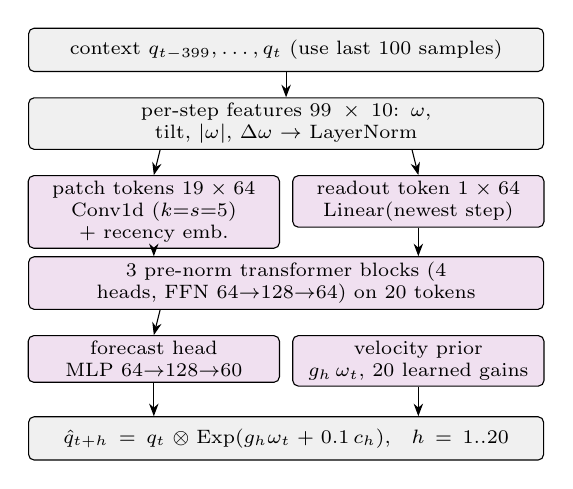
\begin{tikzpicture}[
  box/.style={draw, rounded corners=2pt, align=center, font=\scriptsize, minimum height=0.55cm, inner sep=2pt},
  data/.style={box, fill=gray!12}, learn/.style={box, fill=violet!12}, arr/.style={-{Stealth[length=1.6mm]}, thin},
  node distance=0.32cm]
\node[data, text width=6.4cm] (in) {context $q_{t-399},\dots,q_t$ (use last 100 samples)};
\node[data, text width=6.4cm, below=of in] (feat) {per-step features $99\times10$: $\omega$, tilt, $|\omega|$, $\Delta\omega$ $\rightarrow$ LayerNorm};
\node[learn, text width=3.05cm, below left=0.32cm and -3.2cm of feat] (patch) {patch tokens $19\times64$\\Conv1d ($k{=}s{=}5$) + recency emb.};
\node[learn, text width=3.05cm, below right=0.32cm and -3.2cm of feat] (ro) {readout token $1\times64$\\Linear(newest step)};
\node[learn, text width=6.4cm, below=1.35cm of feat] (enc) {3 pre-norm transformer blocks (4 heads, FFN $64{\to}128{\to}64$) on 20 tokens};
\node[learn, text width=3.05cm, below left=0.32cm and -3.2cm of enc] (head) {forecast head\\MLP $64{\to}128{\to}60$};
\node[learn, text width=3.05cm, below right=0.32cm and -3.2cm of enc] (prior) {velocity prior\\$g_h\,\omega_t$, 20 learned gains};
\node[data, text width=6.4cm, below=1.35cm of enc] (out) {$\hat q_{t+h} = q_t \otimes \mathrm{Exp}(g_h\omega_t + 0.1\,c_h)$, \; $h=1..20$};
\draw[arr] (in) -- (feat);
\draw[arr] (feat.south) ++(-1.6,0) -- (patch.north);
\draw[arr] (feat.south) ++(1.6,0) -- (ro.north);
\draw[arr] (patch.south) -- (patch.south |- enc.north);
\draw[arr] (ro.south) -- (ro.south |- enc.north);
\draw[arr] (enc.south) ++(-1.6,0) -- (head.north);
\draw[arr] (head.south) -- (head.south |- out.north);
\draw[arr] (prior.south) -- (prior.south |- out.north);
\end{tikzpicture}
\caption{\ours. Quaternions become heading-invariant motion features, 50\,ms patch tokens and a readout token; the readout
output drives a residual correction $c_h$ on a learned constant-velocity prior. 121{,}892 parameters.}
\label{fig:arch}
\end{figure}

\textbf{Heading-invariant motion features.} Raw quaternions are dominated by where the player happens to face, which is
arbitrary between sessions, and the per-sample change ($\approx$0.003 per component at 30$^\circ$/s) is tiny compared with
the values themselves. We therefore compute, for consecutive samples, the relative rotation
$\Delta q_t = q_{t-1}^{-1}\otimes q_t$ and the head-frame angular velocity
\begin{equation}
\omega_t \approx 2\,\Delta w_t\,(\Delta x_t, \Delta y_t, \Delta z_t)\, f_s ,
\end{equation}
which is invariant to any global rotation and to the $q/-q$ sign ambiguity, plus the head tilt
$u_t = \mathrm{vec}\bigl(q_t^{-1}\otimes(0,0,1,0)\otimes q_t\bigr)$ (world up seen from the head), which retains pitch and
roll but not the arbitrary yaw. The transformer additionally receives the speed $|\omega_t|$ and the angular acceleration
$\Delta\omega_t$ (10 channels per step, layer-normalised).

\textbf{Tokens.} A strided Conv1d (kernel = stride = 5) turns every 50\,ms into one 64-dimensional token, so the 1\,s
context becomes 19 tokens plus a learned recency (positional) embedding. A readout token, initialised from the newest
step's features, is appended; after three pre-norm blocks~\cite{xiong2020} with GELU~\cite{hendrycks2016}, its output
summarises the history.

\textbf{Residual output on a velocity prior.} The forecast is expressed relative to the newest orientation:
\begin{equation}
\hat q_{t+h} = q_t \otimes \mathrm{Exp}\bigl(g_h\,\omega_t + 0.1\,c_h\bigr),\qquad h = 1,\dots,20,
\end{equation}
where $g_h$ are 20 learned gains (a learned, horizon-dependent damping of constant velocity) and $c_h\in\mathbb{R}^3$ is the
network's correction. The correction head is zero-initialised, so training starts from a sensible kinematic predictor and
learns only the residual motion.

\textbf{Loss.} We optimise the challenge metric directly, written as $2\,\mathrm{atan2}(\|\mathbf{v}\|, |w|)$ of the
relative rotation $\hat q^{-1}\otimes q$ (identical to Eq.~\ref{eq:metric} but with a finite gradient at zero error):
$\mathcal{L} = \overline{\theta_{20}} + \lambda\,\overline{\theta_{1..20}}$ with $\lambda = 0.1$. The all-horizon term
trains the intermediate predictions (Sec.~\ref{sec:ablation}).

\textbf{Training.} AdamW~\cite{loshchilov2019}, one-cycle learning-rate schedule~\cite{smith2019} with peak $10^{-3}$, batch
256, gradient clipping at 1.0, up to 40{,}000 steps with early stopping on validation (evaluation every 1{,}000 steps,
patience 8) \todo{stopped at step X; training time Y min on GPU Z}. The best validation checkpoint is exported.

\textbf{Deployment.} The model is exported to ONNX (opset 17) as a stateless graph: input $[1,400,4]$ quaternions
$(w,x,y,z)$, output $[1,20,4]$ unit quaternions; it reads the last 100 samples. Attention is written with MatMul and Softmax
rather than fused kernels, and quaternion exponentials use a polynomial form (error $<0.002^\circ$ up to $60^\circ$), so the
graph contains only elementary operators. Per prediction it needs 2.20\,M MACs; ONNX and PyTorch outputs agree to
$<10^{-6}$ \todo{confirm from onnx\_checks in metrics.json}.

% =====================================================================================================
\section{Experiments}
\label{sec:results}
\textbf{Protocol.} All models below were trained on the same cache and split and are scored on the \emph{same} 46{,}474
test windows from 1{,}330 held-out users, by running each model's exported ONNX file. Latency is the median single-call time
with ONNX Runtime on one CPU thread \todo{CPU model}; the organisers' XR platform will be slower, but relative ordering is
what the challenge ranks. Differences are tested with a per-user bootstrap (1{,}000 resamples of users, 95\% intervals),
since windows from the same user are correlated~\cite{efron1993}.

\textbf{Compared models.} Physics baselines: last orientation, constant velocity (required by the challenge) and damped
velocity ($\omega$ multiplied by $\beta=0.9$ per step, tuned on training users). Learned models share our input/output design
unless noted: GRU, LSTM, TCN~\cite{bai2018} and a diagonal SSM (S4D-Real~\cite{gu2022s4d}); KalmanNet~\cite{revach2022} on an
angular-velocity/acceleration filter; head-only adaptations of QuaterNet~\cite{pavllo2018}, MOUNT~\cite{chen2024mount} and
controlled residual learning~\cite{yoon2022}, which keep their own architectures; and PoseGRT, a 1.3\,M-parameter
encoder--decoder transformer inspired by GRT~\cite{huang2025grt} (spectral DFT tokens, Perceiver-style horizon queries,
speed and mirror augmentation).

\begin{table}[t]
\caption{Test results (46{,}474 windows, 1{,}330 unseen users). Error in degrees; lower is better for all columns.}
\label{tab:main}
\centering\scriptsize
\setlength{\tabcolsep}{3pt}
\begin{tabular}{lrrrrrr}
\toprule
Model & @200\,ms & @100\,ms & p95 & Params & MACs & ms \\
\midrule
Last orientation      & 6.618 & 3.777 & 16.82 & 0 & 0 & -- \\
Constant velocity     & 7.479 & 3.227 & 19.19 & 0 & 620 & -- \\
Damped velocity       & 5.584 & 2.771 & 13.95 & 2 & 680 & -- \\
\midrule
KalmanNet             & 5.131 & 2.581 & 12.74 & 140k & 13.7M & 7.42 \\
QuaterNet (adapt.)    & 4.903 & 2.463 & 12.01 & 151k & 17.7M & 1.61 \\
Ctrl.\ residual (adapt.) & 4.788 & 2.417 & 11.75 & 270k & 2.1M & 0.92 \\
TCN                   & 4.702 & 2.787 & 11.51 & 49k & 3.7M & 0.25 \\
SSM (S4D)             & 4.688 & 2.787 & 11.52 & 34k & 2.1M & 0.40 \\
LSTM                  & 4.676 & 2.787 & 11.46 & 83k & 6.5M & 0.34 \\
GRU                   & 4.639 & 2.787 & 11.37 & 66k & 4.9M & 0.33 \\
MOUNT (adapt.)        & 4.598 & 2.250 & 11.26 & 294k & 20.4M & 0.82 \\
GRU-128, context 200  & 4.506 & 2.246 & 11.07 & 223k & 39.3M & 1.43 \\
PoseGRT (GRT-style)   & \textbf{4.413} & \textbf{2.203} & \textbf{10.75} & 1.34M & 78.2M & 2.11 \\
\midrule
\textbf{\ours\ (submitted)} & 4.517 & 2.237 & 11.09 & 122k & 2.2M & \textbf{0.25} \\
\bottomrule
\end{tabular}
\end{table}

\textbf{Main result.} Table~\ref{tab:main} lists the results. \ours\ reduces the error of the constant-velocity baseline by
39.6\% (7.48$^\circ\!\to$4.52$^\circ$) and of damped velocity by 19.1\%; the per-user bootstrap interval of the improvement
over damped velocity is [1.03, 1.11]$^\circ$. Only two models are more accurate: PoseGRT (by 0.09--0.12$^\circ$, 95\%
interval) at 11$\times$ the parameters, 36$\times$ the MACs and 8.6$\times$ the latency, and a 157k-parameter variant of
\ours\ with a 2\,s context (4.475$^\circ$) at 1.6$\times$ the latency. Ranking our candidates on accuracy, latency and
parameters with the challenge weights (40/30/10), \ours\ has the best combined rank, which is why we submit it.
Fig.~\ref{fig:tradeoff} shows the trade-off.

\begin{figure}[t]
\centering
\IfFileExists{figs/fig_tradeoff.pdf}{\includegraphics[width=\columnwidth]{figs/fig_tradeoff.pdf}}{\fbox{fig\_tradeoff.pdf}}
\caption{Accuracy versus ONNX latency (marker area $\propto$ log parameters). \ours\ sits at the efficient frontier; larger
models buy at most 0.1$^\circ$ with an order of magnitude more compute.}
\label{fig:tradeoff}
\end{figure}

\subsection{Ablations}
\label{sec:ablation}
\textbf{Input representation.} Replacing the motion features with raw quaternions costs the transformer 0.56$^\circ$
(4.475$\to$5.031$^\circ$, +12.4\%) but leaves the GRU unchanged (4.635 vs.\ 4.630$^\circ$). Attention over patch tokens
benefits most from inputs that are already invariant to heading; the recurrent model can learn differences itself.

\textbf{All-horizon loss.} Training on the 20th sample only ($\lambda=0$) leaves the first 19 outputs at the initial prior:
all four $\lambda{=}0$ sequence models score exactly 2.787$^\circ$ at 100\,ms, slightly \emph{worse} than damped velocity,
followed by a jump at 200\,ms. With $\lambda=0.1$ the GRU's 100\,ms error drops to 2.301$^\circ$ at an unchanged score
(4.639$\to$4.635$^\circ$), yielding smooth, physically plausible trajectories (Fig.~\ref{fig:horizon}).

\textbf{Capacity, context and training length.} Doubling the GRU width (66k$\to$223k parameters) gains 0.06$^\circ$; doubling
its context to 2\,s gains another 0.07$^\circ$ at twice the MACs (8$\times$ those of the base GRU). Training \ours\ for up to 40k steps instead of the
initial run improved it from 4.554 to 4.517$^\circ$ at identical cost. Architecture family matters little: GRU, LSTM, TCN and
SSM with the same inputs and outputs lie within 0.06$^\circ$.

\begin{figure}[t]
\centering
\IfFileExists{figs/fig_horizon.pdf}{\includegraphics[width=\columnwidth]{figs/fig_horizon.pdf}}{\fbox{fig\_horizon.pdf}}
\caption{Mean error versus prediction horizon. Constant velocity overshoots beyond $\approx$150\,ms; learned models stay below
damped velocity at every horizon.}
\label{fig:horizon}
\end{figure}

% =====================================================================================================
\section{Where Does the Remaining Error Come From?}
\label{sec:analysis}
The head rotates on average 6.62$^\circ$ in 200\,ms (the error of the last-orientation predictor); \ours\ leaves
4.52$^\circ$, i.e.\ it anticipates about a third of the motion. Three observations indicate that most of the rest is not
predictable from head motion alone.

\textbf{Convergence.} Ten very different learned architectures converge to 4.4--4.9$^\circ$ (KalmanNet: 5.1$^\circ$), and a
20$\times$ increase in capacity (GRU$\to$PoseGRT) gains only 0.23$^\circ$.

\textbf{Motion regimes.} Grouping windows by the head speed at prediction time (Fig.~\ref{fig:regime}), \ours\ improves on
damped velocity by 9\% when the head is nearly still, 14\% when slow, 24\% when moving and 35\% when fast
(16.43$\to$10.71$^\circ$): the network adds most where extrapolation breaks down. Yet slow windows are 68\% of the data and
contribute most of the error; from a slow or nearly still head, the next 200\,ms often contain the \emph{onset} of a new
movement, triggered by game events or intent that the head trajectory does not reveal.

\textbf{Predictability.} Splitting windows into entropy terciles of the recent trajectory, following~\cite{zhong2025}, the
error rises from 3.52$^\circ$ (easy) to 4.29$^\circ$ (medium) and 5.74$^\circ$ (hard) for \ours, versus 4.29/5.27/7.20$^\circ$
for damped velocity---a consistent 18--20\% improvement in every class.

\begin{figure}[t]
\centering
\IfFileExists{figs/fig_regime.pdf}{\includegraphics[width=\columnwidth]{figs/fig_regime.pdf}}{\fbox{fig\_regime.pdf}}
\caption{Error at 200\,ms by head speed at prediction time (shares of windows: 1.4\%, 67.5\%, 29.0\%, 2.1\%).}
\label{fig:regime}
\end{figure}

Since every competitor faces the same floor, we expect accuracy differences among strong submissions to be small, which
makes latency and size decisive---the reason \ours\ trades 0.1$^\circ$ for an order of magnitude in compute.

% =====================================================================================================
\section{Limitations}
Our data are Beat Saber sessions only; other applications may move differently, and the organisers' test set is not part of
BOXRR-23. Latency was measured on a desktop CPU, not the target XR platform. The exported graph uses operators beyond the
minimal list in the challenge guidelines (e.g.\ Softmax, Sqrt, Split) \todo{check against the Submitting Artifacts page}.
Users are identified by account, so one person with several accounts could appear in two splits. Finally, the model is
stateless and re-reads its 1\,s context at every step; a stateful variant would cut computation further.

% =====================================================================================================
\section{Conclusion}
\ours\ shows that a small transformer over heading-invariant motion tokens, predicting a residual on a learned
constant-velocity prior, captures most of what can be learned about 200\,ms head-pose prediction: it is within 0.1$^\circ$ of a
model 11$\times$ larger while running in 0.25\,ms with 122k parameters. Future work should add information the head trajectory
lacks---e.g.\ controller or eye motion where available---rather than capacity. \todo{code availability statement}

% =====================================================================================================
\begin{thebibliography}{99}\footnotesize
\bibitem{nair2024boxrr} V.~Nair \emph{et al.}, ``Berkeley Open Extended Reality Recordings 2023 (BOXRR-23): 4.7 million
motion capture recordings from 105,000 XR users,'' \emph{IEEE Trans.\ Vis.\ Comput.\ Graph.}, vol.~30, no.~5,
pp.~2239--2246, 2024.
\bibitem{azuma1995} R.~Azuma and G.~Bishop, ``A frequency-domain analysis of head-motion prediction,'' in \emph{Proc.\
SIGGRAPH}, 1995.
\bibitem{lavalle2014} S.~M.~LaValle, A.~Yershova, M.~Katsev, and M.~Antonov, ``Head tracking for the Oculus Rift,'' in
\emph{Proc.\ IEEE ICRA}, 2014.
\bibitem{sola2017} J.~Sol\`a, ``Quaternion kinematics for the error-state Kalman filter,'' arXiv:1711.02508, 2017.
\bibitem{zhong2025} \todo{initials} Zhong, Landfeldt, Alce, and Caltenco, ``Predictability-aware motion prediction for edge XR via high-order error-state Kalman
filtering,'' in \emph{Proc.\ ACM VRST}, 2025, arXiv:2507.13179.
\bibitem{revach2022} G.~Revach, N.~Shlezinger, X.~Ni, A.~L.~Escoriza, R.~J.~G.~van~Sloun, and Y.~C.~Eldar, ``KalmanNet:
Neural network aided Kalman filtering for partially known dynamics,'' \emph{IEEE Trans.\ Signal Process.}, vol.~70,
pp.~1532--1547, 2022.
\bibitem{cho2014} K.~Cho \emph{et al.}, ``Learning phrase representations using RNN encoder--decoder for statistical machine
translation,'' in \emph{Proc.\ EMNLP}, 2014.
\bibitem{hochreiter1997} S.~Hochreiter and J.~Schmidhuber, ``Long short-term memory,'' \emph{Neural Comput.}, vol.~9,
no.~8, pp.~1735--1780, 1997.
\bibitem{bai2018} S.~Bai, J.~Z.~Kolter, and V.~Koltun, ``An empirical evaluation of generic convolutional and recurrent
networks for sequence modeling,'' arXiv:1803.01271, 2018.
\bibitem{gu2022s4d} A.~Gu, K.~Goel, A.~Gupta, and C.~R\'e, ``On the parameterization and initialization of diagonal state
space models,'' in \emph{Proc.\ NeurIPS}, 2022.
\bibitem{vaswani2017} A.~Vaswani \emph{et al.}, ``Attention is all you need,'' in \emph{Proc.\ NeurIPS}, 2017.
\bibitem{pavllo2018} D.~Pavllo, D.~Grangier, and M.~Auli, ``QuaterNet: A quaternion-based recurrent model for human
motion,'' in \emph{Proc.\ BMVC}, 2018.
\bibitem{dosovitskiy2021} A.~Dosovitskiy \emph{et al.}, ``An image is worth 16x16 words: Transformers for image recognition
at scale,'' in \emph{Proc.\ ICLR}, 2021.
\bibitem{huang2025grt} T.~Huang, A.~Prabhakara, C.~Chen, J.~Karhade, D.~Ramanan, M.~O'Toole, and A.~Rowe, ``Towards
foundational models for single-chip radar,'' arXiv:2509.12482, 2025.
\bibitem{xiong2020} R.~Xiong \emph{et al.}, ``On layer normalization in the transformer architecture,'' in \emph{Proc.\
ICML}, 2020.
\bibitem{hendrycks2016} D.~Hendrycks and K.~Gimpel, ``Gaussian error linear units (GELUs),'' arXiv:1606.08415, 2016.
\bibitem{loshchilov2019} I.~Loshchilov and F.~Hutter, ``Decoupled weight decay regularization,'' in \emph{Proc.\ ICLR},
2019.
\bibitem{smith2019} L.~N.~Smith and N.~Topin, ``Super-convergence: Very fast training of neural networks using large learning
rates,'' in \emph{Proc.\ SPIE}, vol.~11006, 2019.
\bibitem{chen2024mount} \todo{authors, title} Chen \emph{et al.}, \emph{IEEE Trans.\ Vis.\ Comput.\ Graph.}, vol.~30,
no.~7, 2024, doi:10.1109/TVCG.2022.3228807.
\bibitem{yoon2022} \todo{authors, title} Yoon \emph{et al.}, in \emph{Proc.\ IEEE ICCE}, 2022,
doi:10.1109/ICCE53296.2022.9730327.
\bibitem{efron1993} B.~Efron and R.~J.~Tibshirani, \emph{An Introduction to the Bootstrap}. Chapman \& Hall, 1993.
\end{thebibliography}

\end{document}
